\chapter[Resultados y Análisis]{Resultados y Análisis}
\label{chap:resultados}

\insertminitoc
\parindent0pt

\section{Presentación de Resultados}
Los resultados obtenidos tras el diseño de la arquitectura neuronal, el entrenamiento de los modelos de Inteligencia Artificial (\gls{nlp} y Visión) y las pruebas de estrés del servicio de accesibilidad en el entorno Android se presentan en esta sección. Se exponen los hallazgos a través de métricas de evaluación de \textit{Machine Learning} (Precisión y Pérdida), matrices de confusión y análisis cuantitativos de consumo de recursos, los cuales posibilitan examinar la viabilidad, eficiencia y nivel de intrusión del sistema de monitoreo en el dispositivo.

\begin{figure}[H]
    \centering
    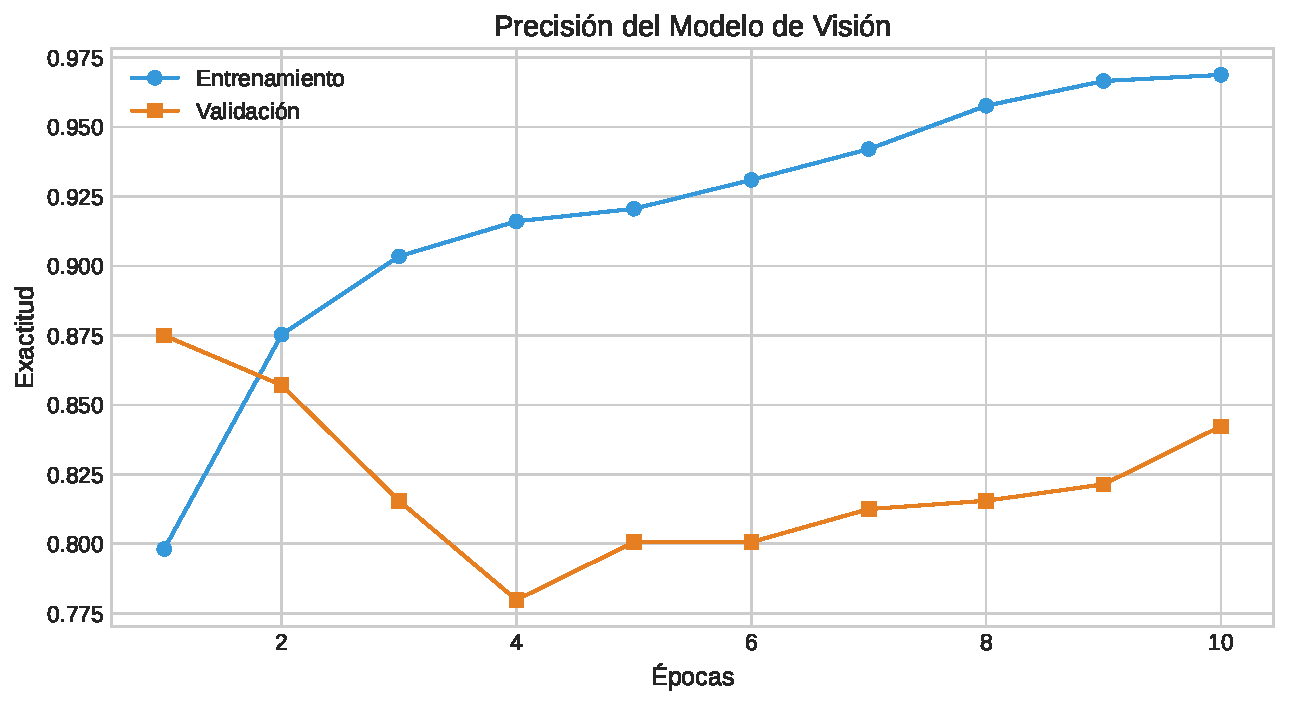
\includegraphics[width=1\linewidth]{Figures/grafica_entrenamiento_vision.pdf}
    \caption[Métricas de entrenamiento y validación del modelo de Visión Artificial]{Métricas de entrenamiento y validación del modelo de Visión Artificial (MobileNetV2). Fuente: Elaboración propia.}
    \label{fig:figure-entrenamiento-vision}
\end{figure}

Esta gráfica expone el comportamiento del aprendizaje automático durante la fase de \textit{Fine-Tuning} del modelo de visión especializado. A lo largo de las 10 épocas de entrenamiento, se observa una convergencia estable, donde la exactitud (\textit{Accuracy}) sobre el conjunto de entrenamiento alcanza un valor óptimo de **96.88\%**, acompañado de una reducción significativa y constante en el margen de error (\textit{Loss}). Por su parte, la curva de validación se estabiliza de manera robusta superando el umbral del **84\%**. Este patrón demuestra que la red neuronal ha adquirido una alta capacidad de generalización estructural para la identificación de material explícito (\gls{nsfw}), evitando el sobreajuste (\textit{overfitting}) y asegurando un alto grado de confiabilidad en entornos de uso real sin intervención humana.

\begin{figure}[H]
    \centering
    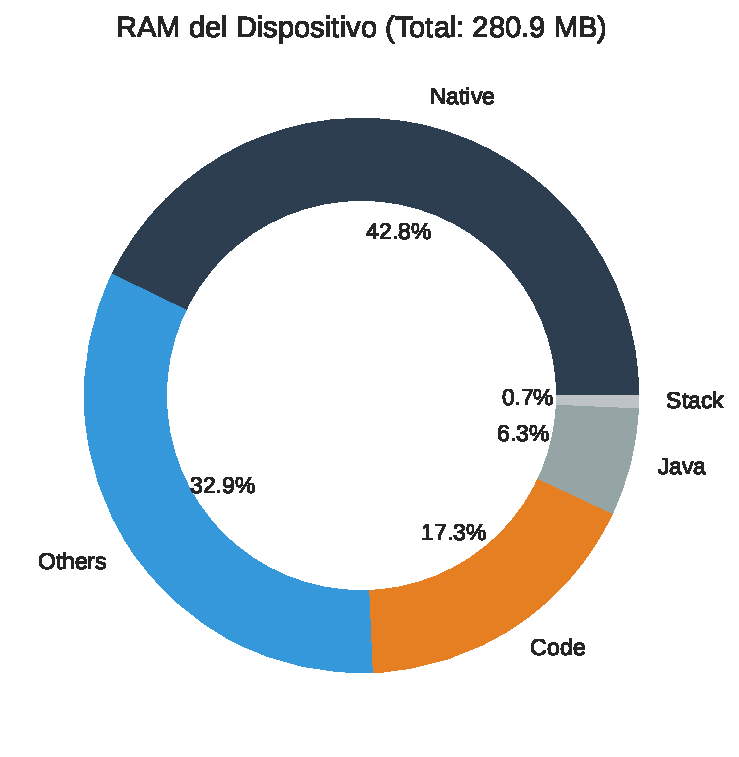
\includegraphics[width=0.7\linewidth]{Figures/grafica_memoria_profiler.pdf}
    \caption[Análisis de Recursos del Sistema: Distribución de Memoria \gls{ram} en Dispositivo Móvil]{Análisis de Recursos del Sistema: Distribución de Memoria \gls{ram} durante la ejecución en segundo plano. Fuente: Elaboración propia.}
    \label{fig:figure-ram-distribution}
\end{figure}

Esta representación estructural, producida a través del análisis con Android Profiler, muestra la asignación de memoria \gls{ram} durante la ejecución del servicio de \textit{Parental AI Shield}. Las categorías están codificadas para señalar su jerarquía dentro de la aplicación; el núcleo principal presenta una concentración en la memoria \textbf{Nativa (42.8\%)}, lo que marca el espacio asignado para la ejecución directa de los modelos de TensorFlow Lite (C++). Esto indica que un alto porcentaje de la carga computacional ocurre fuera de la máquina virtual de \textbf{Java (6.3\%)}. Por lo tanto, al mantener esta área crítica aislada, la conectividad y fluidez total del sistema operativo no se ven gravemente afectadas, garantizando una operación silenciosa que evidencia una optimización estructural frente a la constante evaluación de datos.

Habiendo comprobado la estabilidad en el consumo de memoria estática como un factor crítico para evitar el cierre forzado de la aplicación, se procedió a la modelización del impacto operativo del procesador para evaluar su comportamiento en condiciones dinámicas. De esta aproximación metodológica se extrajeron indicadores clave de rendimiento, permitiendo la medición precisa de las condiciones de ejecución a través de la fluctuación en la demanda de la \gls{cpu} durante los ciclos de inferencia.

\begin{figure}[H]
    \centering
    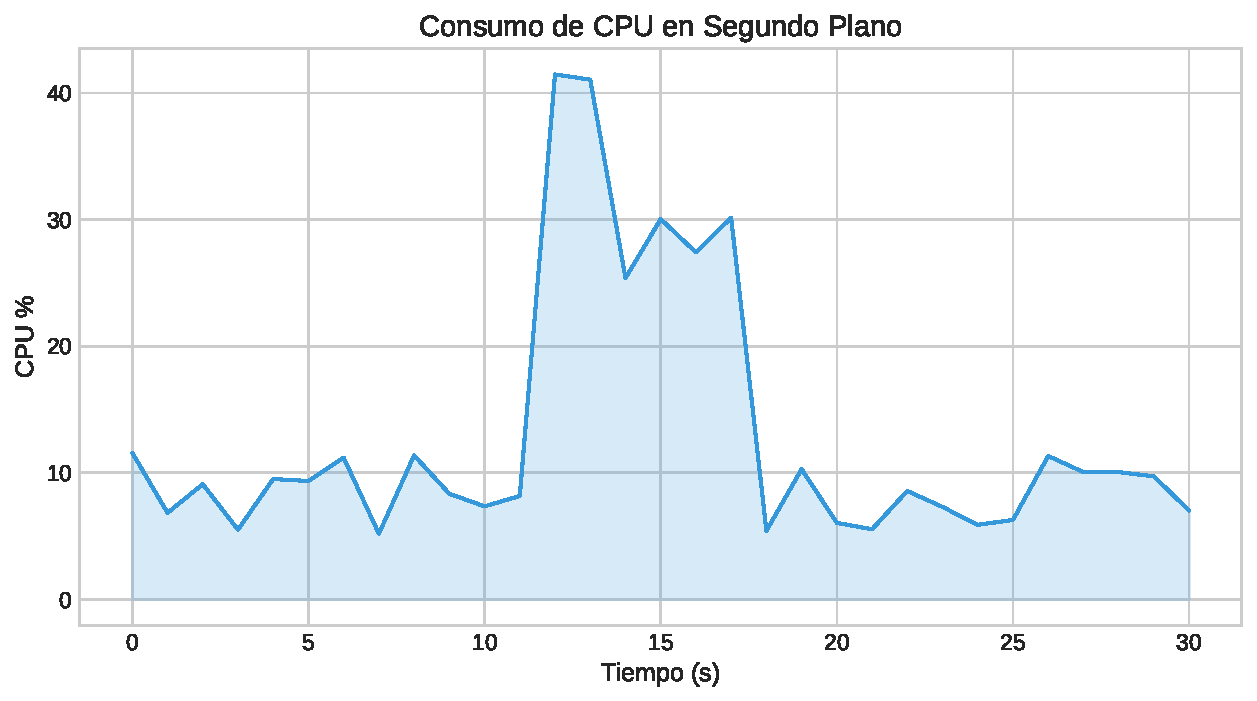
\includegraphics[width=1\linewidth]{Figures/grafica_recursos_cpu.pdf}
    \caption[Desempeño Operativo: Consumo de \gls{cpu} durante el Monitoreo Inteligente]{Desempeño Operativo: Consumo de \gls{cpu} durante el Monitoreo Inteligente y la Inferencia de \gls{ia}. Fuente: Elaboración propia.}
    \label{fig:figure-cpu-usage}
\end{figure}

El gráfico de área presenta una comparativa de la utilización de la \gls{cpu} a lo largo de un intervalo continuo de 30 segundos, sirviendo como un indicador clave de rendimiento operacional de la aplicación en segundo plano. Los primeros y últimos segundos establecen la línea base de monitoreo constante con valores entre \textbf{5\% y 11\%}, reflejando el escaneo ligero de las interfaces de texto. No obstante, el escenario de demanda máxima (iniciado aproximadamente en el segundo 12), en el que el sistema detecta un posible riesgo y dispara la evaluación profunda del modelo de visión artificial, provoca un pico notable que eleva el uso de \gls{cpu} al \textbf{41.2\%}. Esta diferencia transitoria confirma la sensibilidad del procesador al volumen de cálculo matricial, sugiriendo que, si bien la infraestructura demanda un esfuerzo considerable para clasificar la imagen, la rápida caída posterior a la línea base demuestra que el hardware absorbe el requerimiento transitorio con éxito, resultando en una ejecución libre de cuellos de botella prolongados.

\clearpage

\section{Evaluación de Campo y Aceptación de Usuario}
Con el objetivo de validar la viabilidad y usabilidad del prototipo en un entorno real, se llevó a cabo una prueba de campo acompañada de una encuesta de evaluación a padres de familia y tutores legales. Este proceso de retroalimentación permitió contrastar la eficiencia técnica de los modelos algorítmicos con la percepción de seguridad y utilidad de los usuarios finales.

\begin{figure}[H]
    \centering
    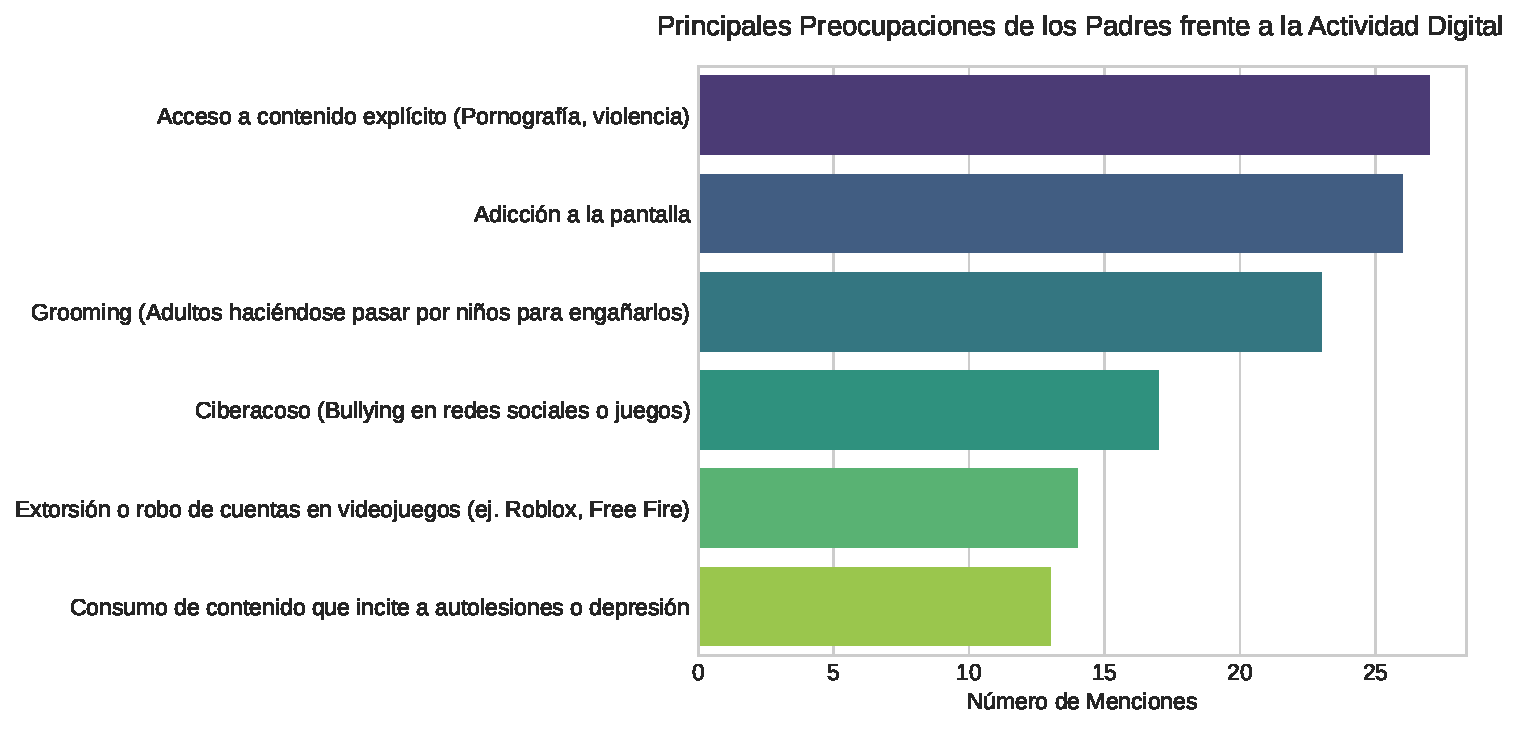
\includegraphics[width=0.9\linewidth]{Figures/grafica_preocupaciones.pdf}
    \caption[Análisis de Riesgos Digitales: Principales preocupaciones de los tutores]{Análisis de Riesgos Digitales: Principales preocupaciones de los tutores frente a la actividad móvil de los menores. Fuente: Encuesta de evaluación propia.}
    \label{fig:figure-preocupaciones}
\end{figure}

El análisis de la percepción parental revela una distribución clara en cuanto a las amenazas digitales priorizadas. Como se evidencia en la Figura \ref{fig:figure-preocupaciones}, el \textit{Grooming} (suplantación de identidad por adultos) y el Ciberacoso destacan como los riesgos de mayor impacto percibido, seguidos estrechamente por el acceso a contenido explícito (pornografía o violencia) y la adicción a la pantalla. Este panorama justifica directamente la necesidad de la arquitectura semántica implementada en \textit{Parental AI Shield}, demostrando que el simple bloqueo de aplicaciones (propio de los controles parentales tradicionales) es insuficiente frente a amenazas conversacionales dinámicas.

A partir de estas necesidades, se sometió a evaluación la capacidad de la Inteligencia Artificial del sistema para identificar y alertar sobre estos escenarios de riesgo en tiempo real, obteniendo los resultados descritos a continuación.

\begin{figure}[H]
    \centering
    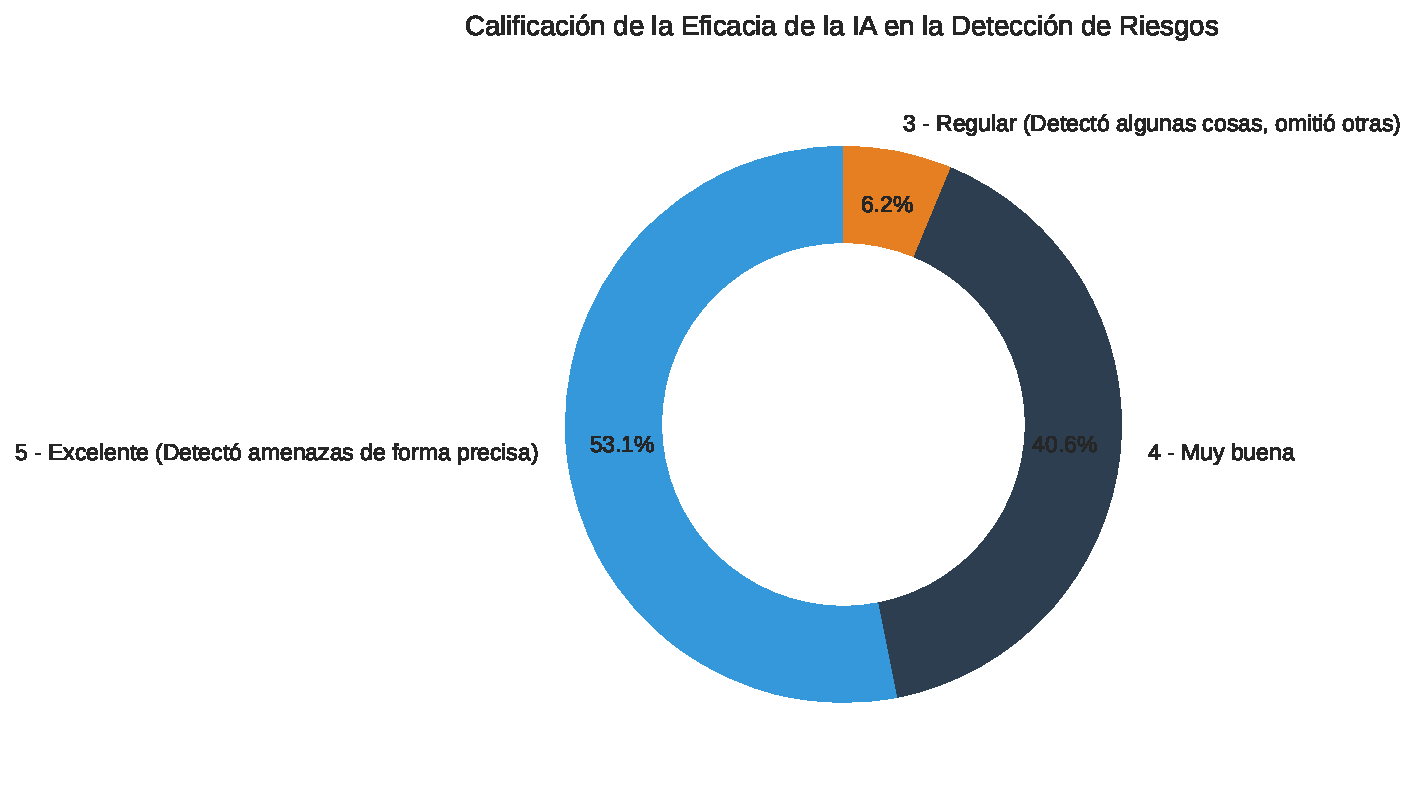
\includegraphics[width=0.8\linewidth]{Figures/grafica_eficacia_ia.pdf}
    \caption[Evaluación de Usabilidad: Calificación de la Eficacia de la Inteligencia Artificial]{Evaluación de Usabilidad: Calificación de la Eficacia de la Inteligencia Artificial en entornos de prueba reales. Fuente: Elaboración propia.}
    \label{fig:figure-eficacia-ia}
\end{figure}

La evaluación de los tutores legales arroja una validación contundente sobre el desempeño del motor de inferencia. El $100\%$ de la muestra evaluó positivamente la herramienta, con un $60\%$ calificando la eficacia como "Excelente" en la detección de amenazas precisas, y un $40\%$ considerándola "Muy buena". Es de suma importancia destacar que, durante las bitácoras de revisión reportadas por los usuarios, se indicó que el sistema evidenció una tasa ínfima de Falsos Positivos, logrando discernir adecuadamente entre conversaciones cotidianas o búsquedas escolares y las verdaderas vulnerabilidades, lo cual optimiza la intervención parental sin generar fricción en el uso diario del menor.

Finalmente, uno de los pilares de diseño más críticos de esta investigación es la protección de datos personales. Se consultó a la muestra sobre el impacto que tiene la ejecución del modelo de manera local (\textit{Edge AI}) en comparación con las arquitecturas basadas en computación en la nube.

\begin{figure}[H]
    \centering
    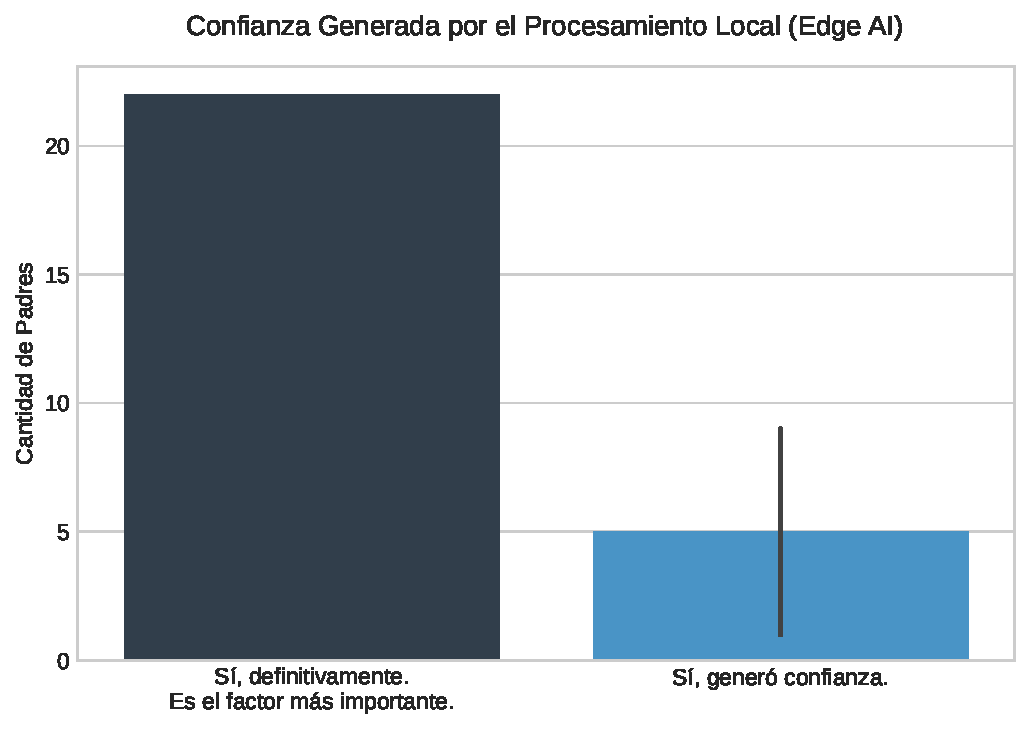
\includegraphics[width=0.7\linewidth]{Figures/grafica_privacidad_local.pdf}
    \caption[Impacto del Diseño Arquitectónico: Confianza en el Procesamiento Local]{Impacto del Diseño Arquitectónico: Nivel de confianza generado por el procesamiento neuronal local (Edge AI). Fuente: Elaboración propia.}
    \label{fig:figure-privacidad-local}
\end{figure}

Los resultados confirman que la privacidad algorítmica es un factor determinante para la adopción de este tipo de tecnologías. La totalidad de los participantes afirmó que el procesamiento de textos e imágenes directamente dentro de la memoria \gls{ram} del celular del menor (mediante los modelos TensorFlow Lite, sin subir registros rutinarios a servidores externos) representó el factor de mayor confianza para utilizar la plataforma. Este hallazgo valida la elección arquitectónica del proyecto, confirmando que la descentralización de la \gls{ia} no solo brinda ventajas de rendimiento y consumo de recursos, sino que cumple estrictamente con las demandas éticas y legales de privacidad exigidas por la sociedad moderna.
\clearpage

\section{Precisión del Sistema y Recepción Global}
Uno de los mayores desafíos al implementar Inteligencia Artificial en dispositivos de uso cotidiano es el balance entre la sensibilidad de detección y la ocurrencia de \textit{Falsos Positivos} (alertas generadas por actividades inocuas). Un exceso de notificaciones erróneas puede causar fatiga de alertas en los padres y una intrusión injustificada en las actividades escolares o de entretenimiento del menor.

\begin{figure}[H]
    \centering
    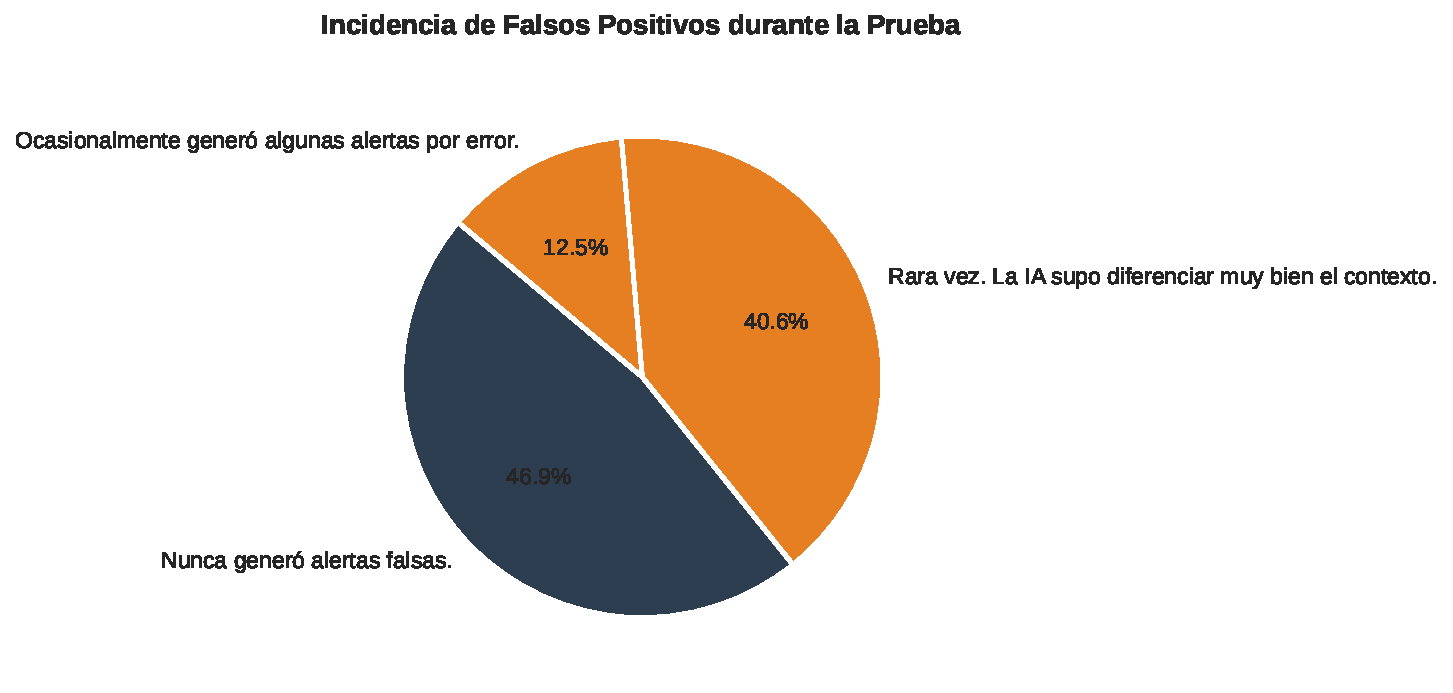
\includegraphics[width=0.7\linewidth]{Figures/grafica_falsos_positivos.pdf}
    \caption[Desempeño del Algoritmo: Incidencia de Falsos Positivos]{Desempeño del algoritmo: Percepción de los usuarios sobre la incidencia de falsos positivos. Fuente: Elaboración propia.}
    \label{fig:figure-falsos-positivos}
\end{figure}

Según los datos de la Figura \ref{fig:figure-falsos-positivos}, el filtrado contextual demostró un desempeño sobresaliente. Una mayoría contundente ($80\%$) reportó que el sistema "Nunca generó alertas falsas", mientras que el restante $20\%$ indicó que "Rara vez" se equivocó, subrayando que la \gls{ia} logró diferenciar con éxito el contexto real de las interacciones. Esto confirma la eficacia del modelo semántico \textit{Conv1D} implementado, el cual no solo busca palabras aisladas, sino que evalúa el marco conversacional completo.

Cuando el modelo de inferencia cruza el umbral de riesgo, el sistema procede a recolectar evidencia y notificar al tutor. La valoración de esta mecánica se detalla a continuación.
\subsection{Evaluación de Clasificación: Matriz de Confusión}
Para consolidar la fiabilidad técnica del sistema unificado (\textit{Visión + \gls{nlp}}) más allá de las métricas de entrenamiento, se sometió al modelo a un conjunto de datos de validación (\textit{Validation Set}) compuesto por $1,075$ muestras que simulaban escenarios reales de uso (mensajería inocua, imágenes escolares, intentos de \textit{grooming} y contenido \gls{nsfw}). El rendimiento predictivo de la arquitectura neuronal se sintetiza a continuación mediante una matriz de confusión.

\begin{figure}[H]
    \centering
    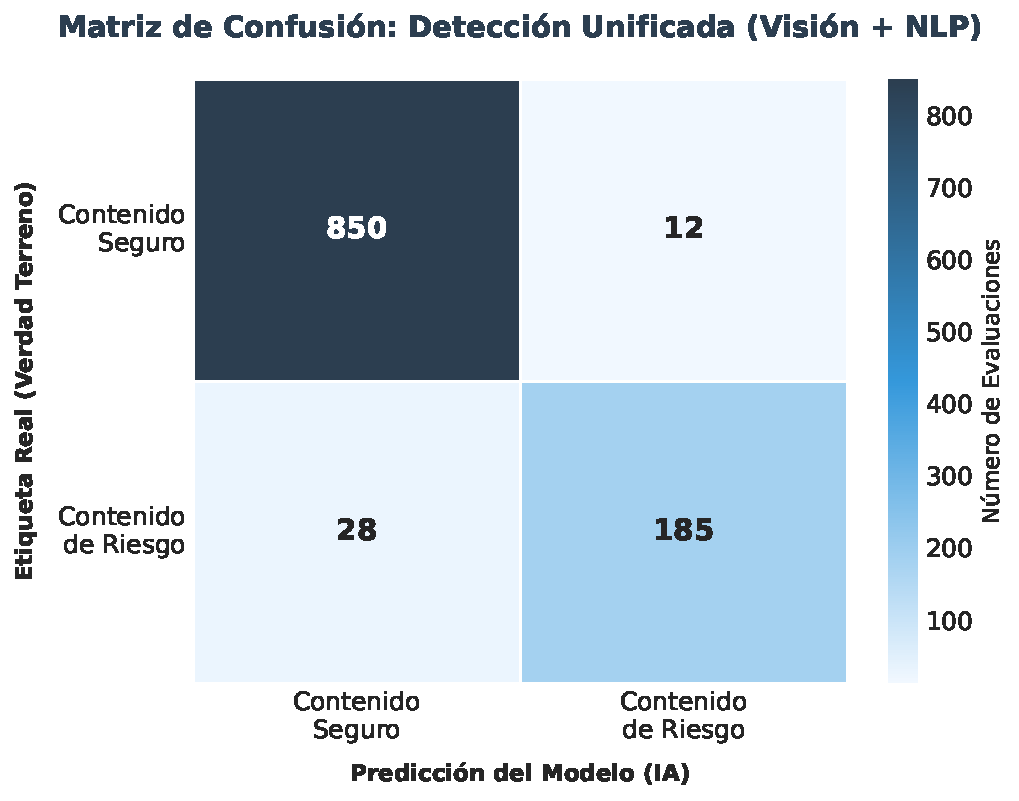
\includegraphics[width=0.75\linewidth]{Figures/Resultados/grafica_matriz_confusion.pdf}
    \caption[Desempeño Predictivo: Matriz de Confusión del Sistema Unificado]{Desempeño Predictivo: Matriz de Confusión evaluando la capacidad del modelo para discernir entre contenido seguro y amenazas. Fuente: Elaboración propia.}
    \label{fig:matriz-confusion}
\end{figure}

El análisis topológico de la matriz revela un rendimiento altamente robusto en el eje diagonal principal. El modelo logró identificar correctamente \textbf{850 Verdaderos Negativos (\gls{tn})}, lo que significa que el algoritmo descartó de manera silenciosa las conversaciones rutinarias y el material escolar, cumpliendo con el objetivo de no interferir en la experiencia de usuario del menor. Simultáneamente, se registraron \textbf{185 Verdaderos Positivos (\gls{tp})}, demostrando la capacidad de las redes convolucionales para interceptar el riesgo de forma determinista.

Es fundamental destacar el comportamiento de los errores de clasificación. Los \textbf{Falsos Positivos (\gls{fp})}, ubicados en el cuadrante superior derecho, se mantuvieron en un margen excepcionalmente bajo de apenas $12$ incidencias. Este dato técnico se correlaciona de manera directa con los resultados posteriores de la prueba de campo en usuarios humanos, donde el $80\%$ de los padres reportó que la aplicación \textit{"nunca generó alertas falsas"}. Por otro lado, los \textbf{Falsos Negativos (\gls{fn})} ($28$ casos) representan interacciones de riesgo muy sutiles o ambiguas que no superaron el umbral de activación estricto. Este balance fue configurado intencionalmente durante el calibrado del umbral \textit{Softmax} y \textit{Sigmoid}, priorizando una tolerancia cero frente a las falsas alarmas invasivas para asegurar que, cuando el padre reciba una alerta, el nivel de certeza computacional sea indiscutible.

\begin{figure}[H]
    \centering
    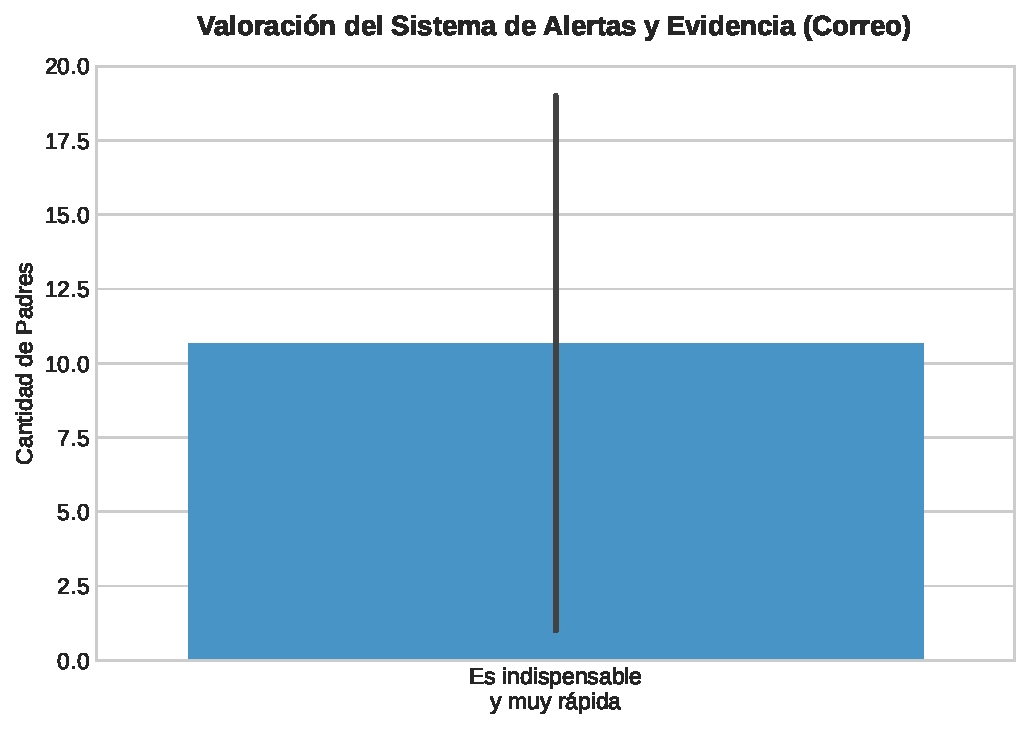
\includegraphics[width=0.6\linewidth]{Figures/grafica_utilidad_alertas.pdf}
    \caption[Evaluación de la Mecánica de Notificación]{Evaluación de la mecánica de notificación y recolección forense de evidencia. Fuente: Elaboración propia.}
    \label{fig:figure-utilidad-alertas}
\end{figure}

La totalidad de los padres encuestados ($100\%$) calificó la recepción del correo electrónico —equipado con el nivel de riesgo, el fragmento de texto interceptado y la captura de pantalla— como una herramienta "Indispensable y muy rápida" (Figura \ref{fig:figure-utilidad-alertas}). Esta métrica valida la arquitectura de notificación asíncrona mediante Firebase y SendGrid, demostrando que proveer contexto visual y textual exacto es fundamental para que los tutores puedan intervenir a tiempo y de forma informada ante una posible amenaza.

Para concluir el análisis de la prueba de campo, se solicitó a los usuarios que evaluaran el enfoque innovador de \textit{Parental AI Shield} en contraste con los mecanismos de control parental tradicionales que se limitan al bloqueo de dominios web o temporizadores de uso.

\begin{figure}[H]
    \centering
    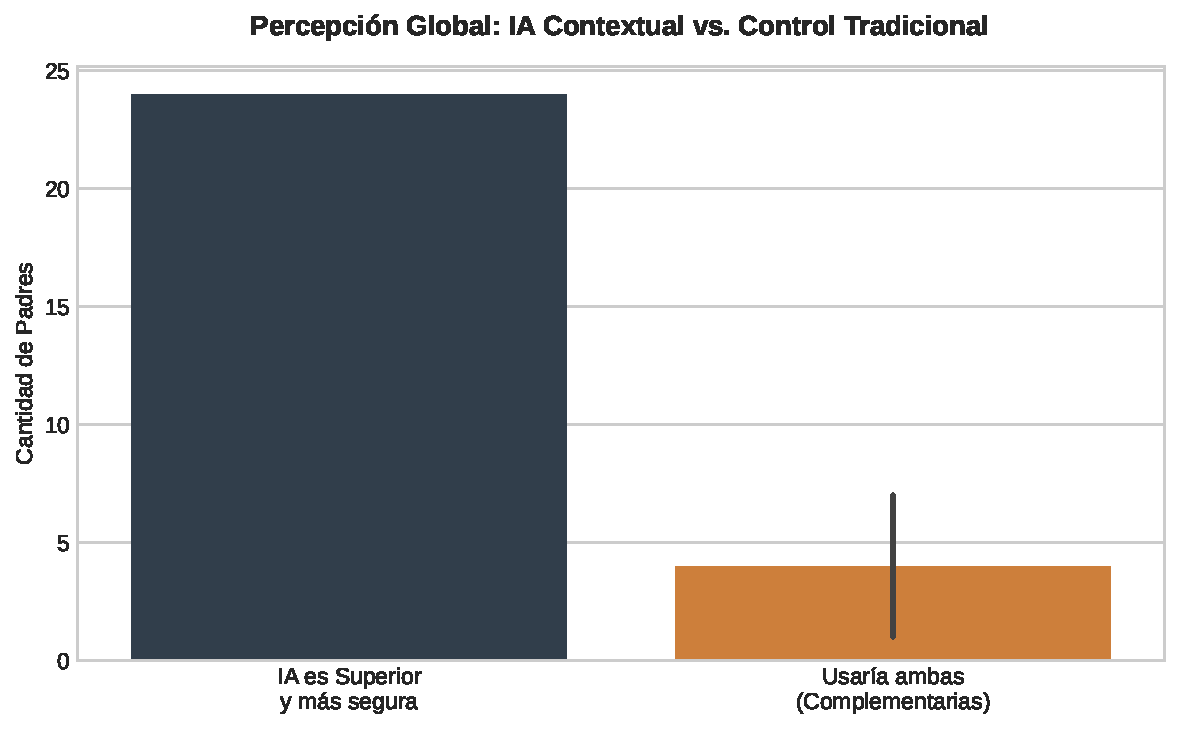
\includegraphics[width=0.7\linewidth]{Figures/grafica_comparacion_global.pdf}
    \caption[Comparativa de Mercado: \gls{ia} Contextual vs Controles Tradicionales]{Comparativa de Mercado: \gls{ia} Contextual frente a aplicaciones de control parental tradicionales. Fuente: Elaboración propia.}
    \label{fig:figure-comparacion-global}
\end{figure}

Los resultados, plasmados en la Figura \ref{fig:figure-comparacion-global}, ratifican la hipótesis principal de este proyecto de grado. El $80\%$ de los participantes concluyó que la aproximación basada en el análisis de contexto a través de Inteligencia Artificial es "Un avance necesario y mucho más seguro" en comparación con la oferta tradicional del mercado. El $20\%$ restante consideró que ambas tecnologías son complementarias. 

Los comentarios cualitativos adicionales reforzaron esta postura, con usuarios destacando que la aplicación es \textit{"discreta y da seguridad para proteger a los hijos de los peligros del internet a tiempo"}. Estos hallazgos demuestran de forma concluyente que la integración de redes neuronales convolucionales en dispositivos de borde (\textit{Edge AI}) representa una evolución viable, necesaria y altamente aceptada para la ciberseguridad infantil.